%%%%%%%%%%%%%%%%%%%%%%%%%%%%%%%%%%%%%%%%%
% University/School Laboratory Report
% LaTeX Template
% Version 3.1 (25/3/14)
%
% This template has been downloaded from:
% http://www.LaTeXTemplates.com
%
% Original author:
% Linux and Unix Users Group at Virginia Tech Wiki 
% (https://vtluug.org/wiki/Example_LaTeX_chem_lab_report)
%
% License:
% CC BY-NC-SA 3.0 (http://creativecommons.org/licenses/by-nc-sa/3.0/)
%
%%%%%%%%%%%%%%%%%%%%%%%%%%%%%%%%%%%%%%%%%

%----------------------------------------------------------------------------------------
%	PACKAGES AND DOCUMENT CONFIGURATIONS
%----------------------------------------------------------------------------------------

\documentclass{article}

\usepackage{array}
\usepackage{tabularx}
\usepackage{geometry}
\usepackage{graphicx} % Required for the inclusion of images
\usepackage[utf8]{inputenc}
\usepackage[english]{babel}
\usepackage{minted}
\usemintedstyle{borland}
\usepackage{xcolor}
\setlength\parindent{1.2pt} % Removes all indentation from paragraphs

\renewcommand{\labelenumi}{\alph{enumi}.} % Make numbering in the enumerate environment by letter rather than number (e.g. subsection 6)
\geometry{
 a4paper,
 total={170mm,257mm},
 left=20mm,
 top=20mm,
 }
%\usepackage{times} % Uncomment to use the Times New Roman font

%----------------------------------------------------------------------------------------
%	DOCUMENT INFORMATION
%----------------------------------------------------------------------------------------

\title{
	Microcontroller Lab Report \\
\large 8086 programming Part 2c
} % Title

\author{
	Aaditya Prakash Kattekola \\
	{\small Roll: 194201} \\
	{\small ECE Section B} \\
} % Author name

\date{August 28, 2021} % Date for the report

\begin{document}

\maketitle % Insert the title, author and date

% If you wish to include an abstract, uncomment the lines below
% \begin{abstract}
% Abstract text
% \end{abstract}

%----------------------------------------------------------------------------------------
%	Question 1
%----------------------------------------------------------------------------------------

\break
\section{Question 1}
%----------------------------------------------------------------------------------------
%	subsection 1
%----------------------------------------------------------------------------------------

\subsection{Aim}
Write an assembly language program for 8086 processor find the largest number in a array. Length of the array is N. Where N represent the last 2 digits of your roll number. 
(Since array of length 01 is not ideal, I used array of length 5)
%----------------------------------------------------------------------------------------
%	subsection 2
%----------------------------------------------------------------------------------------

\subsection{Program}
\subsubsection{Code}
\inputminted{nasm}{"C:/Users/aadit/Documents/BTech/5th Semester/MC Lab/8086 Pgrm 2/2C/MAX_ELEMENT.asm"}

\subsubsection{Emulator}

\begin{center}
\begin{tabularx}{1.0\textwidth} { 
  | >{\centering\arraybackslash}X 
  | >{\centering\arraybackslash}X 
  | >{\centering\arraybackslash}X | }
 \hline
\textbf{Address  (CS:0100, IP:0000)} &\textbf{Machine code}&\textbf{Instruction} \\
  \hline
 01000 & B1, 05 & MOV CL, 05H \\ 
  \hline
  01002 & BE, 00, C9 & MOV 0C900H \\
  \hline
  01005 & BA, 00, 00 & MOV DX, 00000H \\
  \hline
  01008 & 8A, 04 & MOV AL, [SI] \\
  \hline
  0100A & 3A, D0 & CMP DL, AL \\
  \hline 
  0100C & 73, 02 & JNB 010H \\
  \hline
  0100E & 8A, D0 & MOV DL, AL \\
  \hline
  01010 & 46 & INC SI \\
  \hline
  01011 & F8 & CLC \\
  \hline
  01012 & FE, C9 & DEC CL \\
  \hline
  01014 & 75, F2 & JNE 0108H \\
  \hline
 01016 & F4 & HLT \\  
  \hline
\end{tabularx}
\end{center}

%----------------------------------------------------------------------------------------
%	subsection 3
%----------------------------------------------------------------------------------------
\break
\subsection{Result}
\subsubsection{Input}
\begin{figure}[h]
\begin{center}
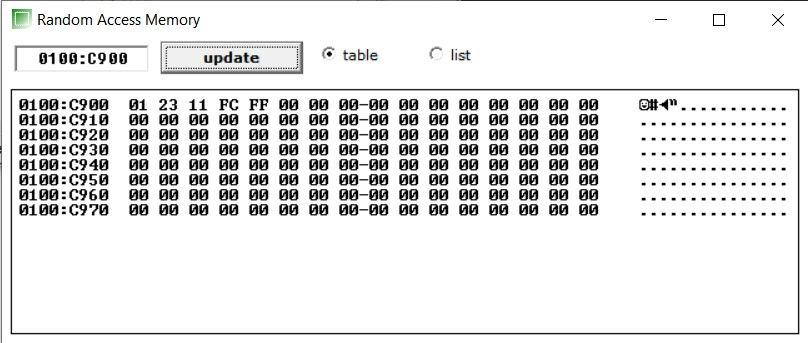
\includegraphics[width=0.8\textwidth]{MAX_ELEMENT_IN} 
\caption{RAM Input for Q1}
\end{center}
\end{figure}

\subsubsection{Expectation}
$ 
Final\ Ans:\  FF\ in\ DX
$ 

%----------------------------------------------------------------------------------------
%	subsection 4
%----------------------------------------------------------------------------------------
\break
\subsubsection{Emulator}

\begin{figure}[h]
\begin{center}
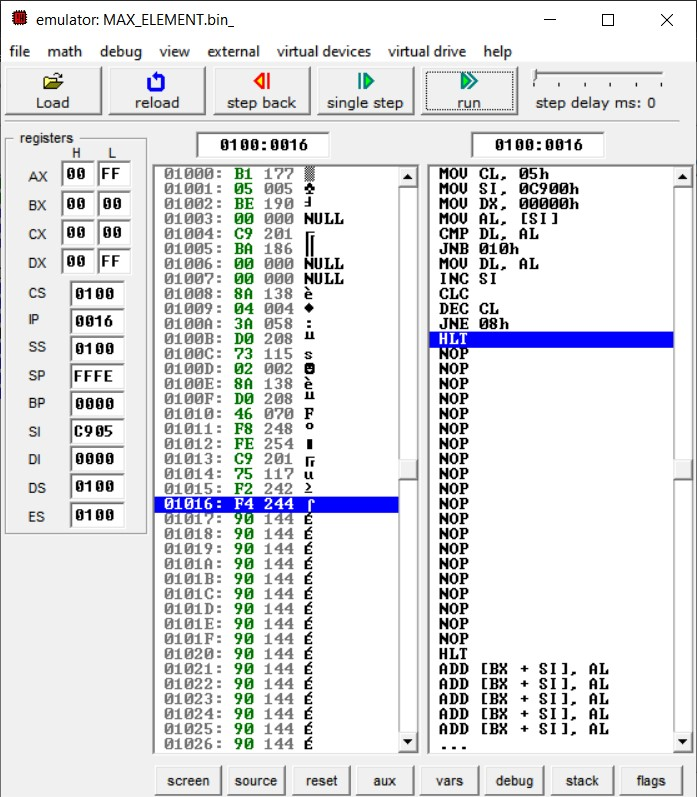
\includegraphics[width=0.75\textwidth]{MAX_ELEMENT_OUT} 
\caption{STACK Output for Q1}
\end{center}
\end{figure}


%----------------------------------------------------------------------------------------
%	Question 2
%----------------------------------------------------------------------------------------

\break
\section{Question 2}
%----------------------------------------------------------------------------------------
%	subsection 1
%----------------------------------------------------------------------------------------

\subsection{Aim}
Write an assembly language program for 8086 processor to calculate LCM of two 8 bit numbers.
%----------------------------------------------------------------------------------------
%	subsection 2
%----------------------------------------------------------------------------------------

\subsection{Program}
\subsubsection{Code}
\inputminted{nasm}{"C:/Users/aadit/Documents/BTech/5th Semester/MC Lab/8086 Pgrm 2/2C/LCM.asm"}

\subsubsection{Emulator}

\begin{center}
\begin{tabularx}{1.0\textwidth} { 
  | >{\centering\arraybackslash}X 
  | >{\centering\arraybackslash}X 
  | >{\centering\arraybackslash}X | }
 \hline
\textbf{Address  (CS:0100, IP:0000)} &\textbf{Machine code}&\textbf{Instruction} \\
  \hline
 01000 & BE, 00, C9 & MOV SI, 0C900H \\ 
  \hline
  01003 & 0B, 00 & OR AX, [BX + SI] \\
  \hline
 01005 & 03, 00 & ADD AX, [BX + SI] \\
 \hline
  01007 & 01, 00 & ADD [BX + SI], AX \\
  \hline
  01009 & 21, 00 & AND [BX + SI], AX \\
  \hline
  0100B & A1, 03, 00 & MOV AX, [00003H] \\
  \hline
  0100E & 8B, 1E, 05, 00 & MOV BX, [00005H] \\
  \hline
 01012 & 3B, C3 & CMP AX, BX \\
 \hline
  01014 & 74, 13 & JZ 029H \\
  \hline
  01016 & 72, 0E & JB 026H \\
  \hline
  01018 & BA, 00, 00 & MOV DX, 00000H \\
  \hline
  0101B & F7, F3 & DIV BX \\
  \hline
  0101D & 83, FA, 00 & CMP DX, 00H \\
  \hline
  01020 & 74, 07 & JZ 029H \\
  \hline
  01022 & 8B, C2 & MOV AX, DX \\
  \hline
  01024 & EB, EC & JMP 012H \\
  \hline
  01026 & 96 & XCHG AX, BX \\
  \hline
  01027 & EB, EF & JMP 018H \\
  \hline
  01029 & 80, 1E, 07, 00 & MOV [00007H], BX \\
  \hline
  0102D & A1, 03, 00 & MOV AX, [00003H] \\
  \hline
  01030 & 8B, 1E, 05, 00 & MOV BX, [00005H] \\
  \hline
  01034 & F7, E3 & MUL BX \\
  \hline
  01036 & F7, 36, 07, 00 & DIV W.[00007H] \\
  \hline
  0103A & A3, 09, 00 & MOV [00009], AX \\
  \hline
  0103D & 8B, 16, 09, 00 & MOV DX, [00009H] \\
  \hline
 01041 & F4 & HLT \\  
  \hline
\end{tabularx}
\end{center}

%----------------------------------------------------------------------------------------
%	subsection 3
%----------------------------------------------------------------------------------------
\subsection{Result}
\subsubsection{Input}
 \begin{figure}[h]
\begin{center}
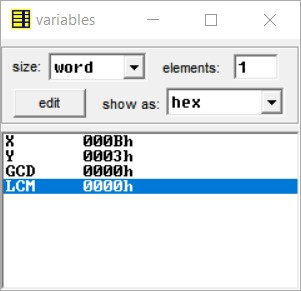
\includegraphics[width=0.45\textwidth]{LCM_IN} 
\caption{VARIABLE Input for Q2 }
\end{center}
\end{figure}
 
\subsubsection{Expectation}
$
 0021H\ (33\ in\ DEC)\ in\ DX 
$ 

%----------------------------------------------------------------------------------------
%	subsection 4
%----------------------------------------------------------------------------------------

\subsubsection{Emulator}
\begin{figure}[h]
\begin{center}
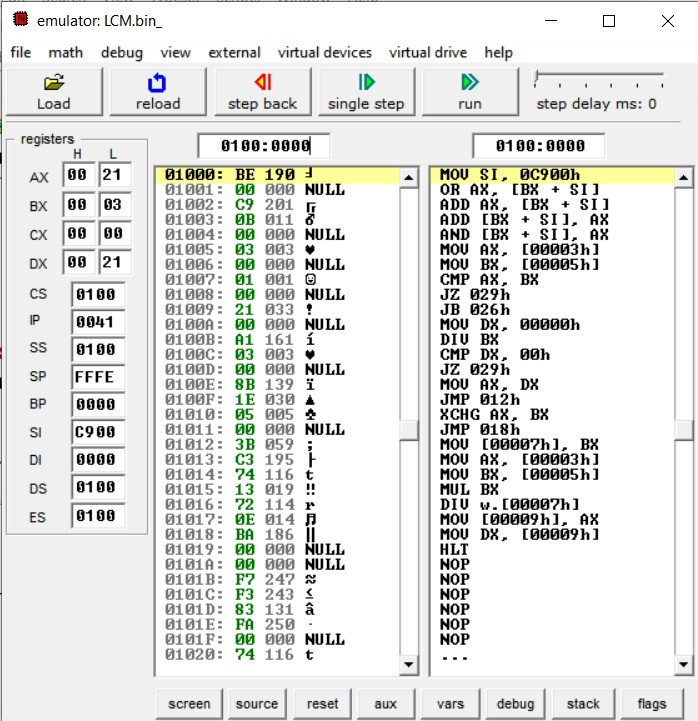
\includegraphics[width=0.7\textwidth]{LCM_OUT1} 
\caption{STACK Output for Q2.1 }
\end{center}
\end{figure}
\begin{figure}[h]
\begin{center}
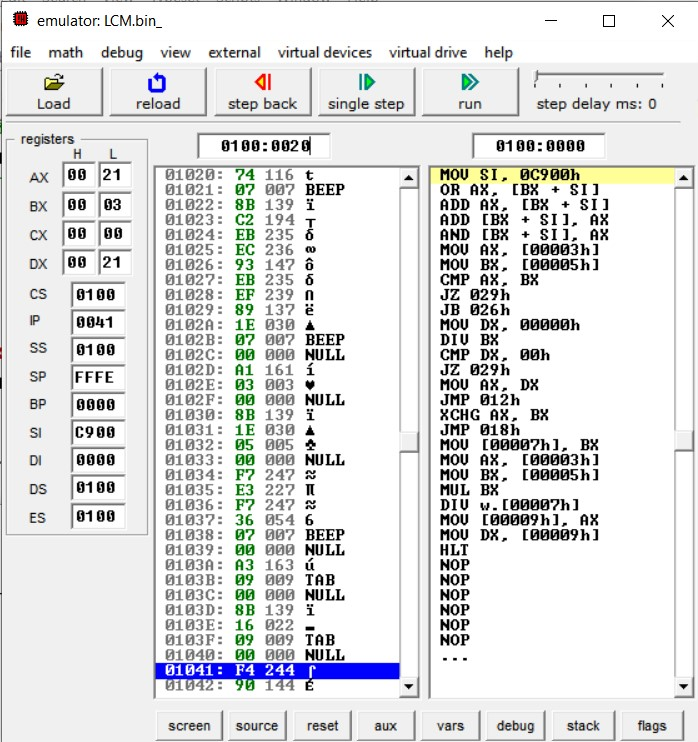
\includegraphics[width=0.7\textwidth]{LCM_OUT2} 
\caption{STACK Output for Q2.2 }
\end{center}
\begin{center}
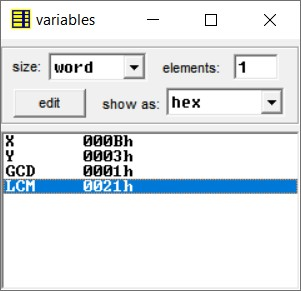
\includegraphics[width=0.45\textwidth]{LCM_OUT3} 
\caption{VARIABLE Output for Q2 }
\end{center}
\end{figure}
\end{document}